% This is the Reed College LaTeX thesis template. Most of the work
% for the document class was done by Sam Noble (SN), as well as this
% template. Later comments etc. by Ben Salzberg (BTS). Additional
% restructuring and APA support by Jess Youngberg (JY).
% Your comments and suggestions are more than welcome; please email
% them to cus@reed.edu
%
% See http://web.reed.edu/cis/help/latex.html for help. There are a
% great bunch of help pages there, with notes on
% getting started, bibtex, etc. Go there and read it if you're not
% already familiar with LaTeX.
%
% Any line that starts with a percent symbol is a comment.
% They won't show up in the document, and are useful for notes
% to yourself and explaining commands.
% Commenting also removes a line from the document;
% very handy for troubleshooting problems. -BTS

% As far as I know, this follows the requirements laid out in
% the 2002-2003 Senior Handbook. Ask a librarian to check the
% document before binding. -SN

%%
%% Preamble
%%
% \documentclass{<something>} must begin each LaTeX document
\documentclass[12pt,twoside]{reedthesis}
% Packages are extensions to the basic LaTeX functions. Whatever you
% want to typeset, there is probably a package out there for it.
% Chemistry (chemtex), screenplays, you name it.
% Check out CTAN to see: http://www.ctan.org/
%%
\usepackage{graphicx,latexsym}
\usepackage{amsmath}
\usepackage{amssymb,amsthm}
\usepackage{longtable,booktabs,setspace}
\usepackage{chemarr} %% Useful for one reaction arrow, useless if you're not a chem major
\usepackage[hyphens]{url}
% Added by CII
\usepackage{hyperref}
\usepackage{lmodern}
\usepackage{float}
\floatplacement{figure}{H}
% End of CII addition
\usepackage{rotating}

% Next line commented out by CII
%%% \usepackage{natbib}
% Comment out the natbib line above and uncomment the following two lines to use the new
% biblatex-chicago style, for Chicago A. Also make some changes at the end where the
% bibliography is included.
%\usepackage{biblatex-chicago}
%\bibliography{thesis}


% Added by CII (Thanks, Hadley!)
% Use ref for internal links
\renewcommand{\hyperref}[2][???]{\autoref{#1}}
\def\chapterautorefname{Chapter}
\def\sectionautorefname{Section}
\def\subsectionautorefname{Subsection}
% End of CII addition

% Added by CII
\usepackage{caption}
\captionsetup{width=5in}
% End of CII addition

% \usepackage{times} % other fonts are available like times, bookman, charter, palatino

% Syntax highlighting #22
  \usepackage{color}
  \usepackage{fancyvrb}
  \newcommand{\VerbBar}{|}
  \newcommand{\VERB}{\Verb[commandchars=\\\{\}]}
  \DefineVerbatimEnvironment{Highlighting}{Verbatim}{commandchars=\\\{\}}
  % Add ',fontsize=\small' for more characters per line
  \usepackage{framed}
  \definecolor{shadecolor}{RGB}{248,248,248}
  \newenvironment{Shaded}{\begin{snugshade}}{\end{snugshade}}
  \newcommand{\KeywordTok}[1]{\textcolor[rgb]{0.13,0.29,0.53}{\textbf{#1}}}
  \newcommand{\DataTypeTok}[1]{\textcolor[rgb]{0.13,0.29,0.53}{#1}}
  \newcommand{\DecValTok}[1]{\textcolor[rgb]{0.00,0.00,0.81}{#1}}
  \newcommand{\BaseNTok}[1]{\textcolor[rgb]{0.00,0.00,0.81}{#1}}
  \newcommand{\FloatTok}[1]{\textcolor[rgb]{0.00,0.00,0.81}{#1}}
  \newcommand{\ConstantTok}[1]{\textcolor[rgb]{0.00,0.00,0.00}{#1}}
  \newcommand{\CharTok}[1]{\textcolor[rgb]{0.31,0.60,0.02}{#1}}
  \newcommand{\SpecialCharTok}[1]{\textcolor[rgb]{0.00,0.00,0.00}{#1}}
  \newcommand{\StringTok}[1]{\textcolor[rgb]{0.31,0.60,0.02}{#1}}
  \newcommand{\VerbatimStringTok}[1]{\textcolor[rgb]{0.31,0.60,0.02}{#1}}
  \newcommand{\SpecialStringTok}[1]{\textcolor[rgb]{0.31,0.60,0.02}{#1}}
  \newcommand{\ImportTok}[1]{#1}
  \newcommand{\CommentTok}[1]{\textcolor[rgb]{0.56,0.35,0.01}{\textit{#1}}}
  \newcommand{\DocumentationTok}[1]{\textcolor[rgb]{0.56,0.35,0.01}{\textbf{\textit{#1}}}}
  \newcommand{\AnnotationTok}[1]{\textcolor[rgb]{0.56,0.35,0.01}{\textbf{\textit{#1}}}}
  \newcommand{\CommentVarTok}[1]{\textcolor[rgb]{0.56,0.35,0.01}{\textbf{\textit{#1}}}}
  \newcommand{\OtherTok}[1]{\textcolor[rgb]{0.56,0.35,0.01}{#1}}
  \newcommand{\FunctionTok}[1]{\textcolor[rgb]{0.00,0.00,0.00}{#1}}
  \newcommand{\VariableTok}[1]{\textcolor[rgb]{0.00,0.00,0.00}{#1}}
  \newcommand{\ControlFlowTok}[1]{\textcolor[rgb]{0.13,0.29,0.53}{\textbf{#1}}}
  \newcommand{\OperatorTok}[1]{\textcolor[rgb]{0.81,0.36,0.00}{\textbf{#1}}}
  \newcommand{\BuiltInTok}[1]{#1}
  \newcommand{\ExtensionTok}[1]{#1}
  \newcommand{\PreprocessorTok}[1]{\textcolor[rgb]{0.56,0.35,0.01}{\textit{#1}}}
  \newcommand{\AttributeTok}[1]{\textcolor[rgb]{0.77,0.63,0.00}{#1}}
  \newcommand{\RegionMarkerTok}[1]{#1}
  \newcommand{\InformationTok}[1]{\textcolor[rgb]{0.56,0.35,0.01}{\textbf{\textit{#1}}}}
  \newcommand{\WarningTok}[1]{\textcolor[rgb]{0.56,0.35,0.01}{\textbf{\textit{#1}}}}
  \newcommand{\AlertTok}[1]{\textcolor[rgb]{0.94,0.16,0.16}{#1}}
  \newcommand{\ErrorTok}[1]{\textcolor[rgb]{0.64,0.00,0.00}{\textbf{#1}}}
  \newcommand{\NormalTok}[1]{#1}

% To pass between YAML and LaTeX the dollar signs are added by CII
\title{Neural Network Methods for Complex Survey Imputation}
\author{Alexander Michael Moore}
% The month and year that you submit your FINAL draft TO THE LIBRARY (May or December)
\date{May 2019}
\division{Mathematics and Statistics}
\advisor{Kelly McConville}
\institution{Reed College}
\degree{Bachelor of Arts}
%If you have two advisors for some reason, you can use the following
% Uncommented out by CII
% End of CII addition

%%% Remember to use the correct department!
\department{Mathematics}
% if you're writing a thesis in an interdisciplinary major,
% uncomment the line below and change the text as appropriate.
% check the Senior Handbook if unsure.
%\thedivisionof{The Established Interdisciplinary Committee for}
% if you want the approval page to say "Approved for the Committee",
% uncomment the next line
%\approvedforthe{Committee}

% Added by CII
%%% Copied from knitr
%% maxwidth is the original width if it's less than linewidth
%% otherwise use linewidth (to make sure the graphics do not exceed the margin)
\makeatletter
\def\maxwidth{ %
  \ifdim\Gin@nat@width>\linewidth
    \linewidth
  \else
    \Gin@nat@width
  \fi
}
\makeatother

\renewcommand{\contentsname}{Table of Contents}
% End of CII addition

\setlength{\parskip}{0pt}

% Added by CII

\providecommand{\tightlist}{%
  \setlength{\itemsep}{0pt}\setlength{\parskip}{0pt}}

\Acknowledgements{
I want to thank a few people.
}

\Dedication{
You can have a dedication here if you wish.
}

\Preface{
This is an example of a thesis setup to use the reed thesis document
class (for LaTeX) and the R bookdown package, in general.
}

\Abstract{
This is my abstract. Packet from unrealeased textbook has great guide
for abstract. \par

Second paragraph of abstract starts here.
}

% End of CII addition
%%
%% End Preamble
%%
%
\begin{document}

% Everything below added by CII
  \maketitle

\frontmatter % this stuff will be roman-numbered
\pagestyle{empty} % this removes page numbers from the frontmatter
  \begin{acknowledgements}
    I want to thank a few people.
  \end{acknowledgements}
  \begin{preface}
    This is an example of a thesis setup to use the reed thesis document
    class (for LaTeX) and the R bookdown package, in general.
  \end{preface}
  \hypersetup{linkcolor=black}
  \setcounter{tocdepth}{2}
  \tableofcontents

  \listoftables

  \listoffigures
  \begin{abstract}
    This is my abstract. Packet from unrealeased textbook has great guide
    for abstract. \par
    
    Second paragraph of abstract starts here.
  \end{abstract}
  \begin{dedication}
    You can have a dedication here if you wish.
  \end{dedication}
\mainmatter % here the regular arabic numbering starts
\pagestyle{fancyplain} % turns page numbering back on

\chapter*{Introduction}\label{introduction}
\addcontentsline{toc}{chapter}{Introduction}

Welcome to the \emph{R Markdown} thesis template. This template is based
on (and in many places copied directly from) the Reed College LaTeX
template, but hopefully it will provide a nicer interface for those that
have never used TeX or LaTeX before. Using \emph{R Markdown} will also
allow you to easily keep track of your analyses in \textbf{R} chunks of
code, with the resulting plots and output included as well. The hope is
this \emph{R Markdown} template gets you in the habit of doing
reproducible research, which benefits you long-term as a researcher, but
also will greatly help anyone that is trying to reproduce or build onto
your results down the road.

Hopefully, you won't have much of a learning period to go through and
you will reap the benefits of a nicely formatted thesis. The use of
LaTeX in combination with \emph{Markdown} is more consistent than the
output of a word processor, much less prone to corruption or crashing,
and the resulting file is smaller than a Word file. While you may have
never had problems using Word in the past, your thesis is likely going
to be about twice as large and complex as anything you've written
before, taxing Word's capabilities. After working with \emph{Markdown}
and \textbf{R} together for a few weeks, we are confident this will be
your reporting style of choice going forward.

\textbf{Why use it?}

\emph{R Markdown} creates a simple and straightforward way to interface
with the beauty of LaTeX. Packages have been written in \textbf{R} to
work directly with LaTeX to produce nicely formatting tables and
paragraphs. In addition to creating a user friendly interface to LaTeX,
\emph{R Markdown} also allows you to read in your data, to analyze it
and to visualize it using \textbf{R} functions, and also to provide the
documentation and commentary on the results of your project. Further, it
allows for \textbf{R} results to be passed inline to the commentary of
your results. You'll see more on this later.

\textbf{Who should use it?}

Anyone who needs to use data analysis, math, tables, a lot of figures,
complex cross-references, or who just cares about the final appearance
of their document should use \emph{R Markdown}. Of particular use should
be anyone in the sciences, but the user-friendly nature of
\emph{Markdown} and its ability to keep track of and easily include
figures, automatically generate a table of contents, index, references,
table of figures, etc. should make it of great benefit to nearly anyone
writing a thesis project.

\chapter{Complex Surveys}\label{complex-surveys}

\section{Survey Statistics}\label{survey-statistics}
\begin{quote}
Researchers in the social science and health sciences are increasingly
interested in using data from complex surveys to conduct the same sorts
of analyses that they traditionally conduct with more straightforward
data. - Lumley 1969
\end{quote}
The implicit pervasiveness of survey statistics in all data motivates
our exploration into its significance in imputation.

Survey statistics differ from statistics modelling in the specification
of the random process that generates the data. In model-based
statistics, some underlying generative model from which observations are
drawn is assumed to exist. By understanding or approximating this model
from data, one may draw conclusions on the nature of the generative
function provided no meaningful changes to the data are made.

Contrary to model-based statistics, the analysis of complex survey
samples are design based. The observations from a researcher-specified
population have fixed features, and randomness is introduced when these
observations are drawn from the population according to some stochastic
design. This random process is under the control of the researcher, and
can be known precisely. The significance of design-based methods is that
the probability sample design is the procedure for taking samples from a
population, not just the resulting data. This is a significant departure
from the statistical analysis mindset that randomness is an element of
the features and labels of a population. Using this method, the features
of the population from which the observations are drawn may be
estimated, but these conclusions may not generalize to other
populations. With understanding of the survey sampling design from which
data observations arise, the researcher may make improved estimates of
the population of study compared to naive estimates (Lumley, 2011).

The probability sample design is the fundamental concept of design-based
inference. Taking a random sample of 36,000 people from Oregon is an
example of a survey design which implies independent and equal
probability sampling of all humans in the state. The Law of Large
Numbers is invoked to assume the distribution of sampled observations
represents the population from which they are drawn according to any
features of interest to the researcher, such as height, weight, or age.

This type of surveying can be complicated by adding unequal inclusion
probability to the features to oversample from minority groups. The data
created by such a design would likely not be representative of the
population, since people with higher inclusion probabilities would be
more likely to be sampled. However, since the probability of each person
in the sample being randomly selected is known (since the population
total is known), this is still a probability sample. The key point of
this process is that a probability sample is the procedure for taking
samples from a population, not a data set (Lumley, 2011).

There are four requirements for a data set to be a probability sample:
\begin{enumerate}
\def\labelenumi{\arabic{enumi}.}
\item
  Every individual in the population must have a non-zero probability of
  ending up in the sample.
\item
  The probability of inclusion must be known for every individual who
  does end up in the sample.
\item
  Every pair of individuals in the sample must have a non-zero
  probability of both ending up in the sample.
\item
  The probability of every pair of individuals being included in the
  sample must be known for every pair of individuals in the sample.
\end{enumerate}
1 and 2 are necessary in order to get valid population estimates, 3 and
4 are necessary to work out the accuracy of the estimates. If
individuals were sampled independently of each other the first two
properties would guarantee the last two (Lumley, 2011). Though 3 and 4
are requirements of a probability sample, they are often not included in
datasets as they require an \(n \times n\) matrix of probabilities,
where \(n\) is the number of observations in the data set.

The fundamental statistical idea behind all of design-based inference is
that an individual sampled with a sampling probability \(\pi_i\)
represents \(\frac{1}{\pi_i}\) individuals in the population. The value
\(\frac{1}{\pi_i}\) is called the sampling weight (Lumley, 2011). Since
observations represent different proportions of the population, the
inclusion probability must be accounted for in modeling and estimation
procedures.

Data collected under a complex survey design have an additional layer of
complexity and are not to be treated as independent and identically
distributed (\emph{i.i.d.}). Ignoring this complex survey design is
found to create significant error in data analyses (Toth \& Eltinge,
2011). This concern motivates our exploration of accounting for survey
design in neural network imputation.

\section{Imputation}\label{imputation}

Often in real-world data, there is some degree of missingness. This can
be for any number of reasons, illustrated below:
\begin{verbatim}

Attaching package: 'kableExtra'
\end{verbatim}
\begin{verbatim}
The following object is masked from 'package:dplyr':

    group_rows
\end{verbatim}
\begin{table}[t]

\caption{\label{tab:missingness}Types of missingess}
\centering
\begin{tabular}{l|l}
\hline
  & Description\\
\hline
Noncoverage & An element in the target population is not included in the survey sampling frame\\
\hline
Total Nonresponse & A sampled element does not participate in the survey\\
\hline
Item Nonresponse & A responding sampled element fails to provide acceptable responses to one or more of the survey items\\
\hline
\end{tabular}
\end{table}
Item nonresponse is the focus of this thesis. Item nonresponse will be
restricted to a response value of interest called a label and will be
present in some of the observations. The other variables of the
observation, called features, will be fully present. The usual form of
handling item nonresponse is imputation, which fills in missing values
with usable information (Brick \& Kalton, 1996). Common algorithms such
as Principal Component Analysis and regression require no missingness in
the data set, so replacing NA values with useable information is vital
for analysis.

In many statistical analyses, observations with any degree of
missingness cannot be included. For example, how would one perform a
linear regression with observations that have features but no label?
Dropping these terms would remove potentially huge swathes of the data
set, particularly in multivariate data sets, and would potentially
create systematic bias.

Suppose for example a data set with information on roses had a feature
with stem length and a label on flower size measured by a researcher.
There might be missing values for flower size that are not randomly
distributed: Before the researcher makes measurements, there has been
systematic removal of the large-flowered roses by passersby. To ignore
these observations would lead the analyst to draw false conclusions on
the relationship of stem length to flower size, the distribution of
flower sizes in the population, and estimations of the mean flower size
in the population of all flowers, visualized in Example 1.1:

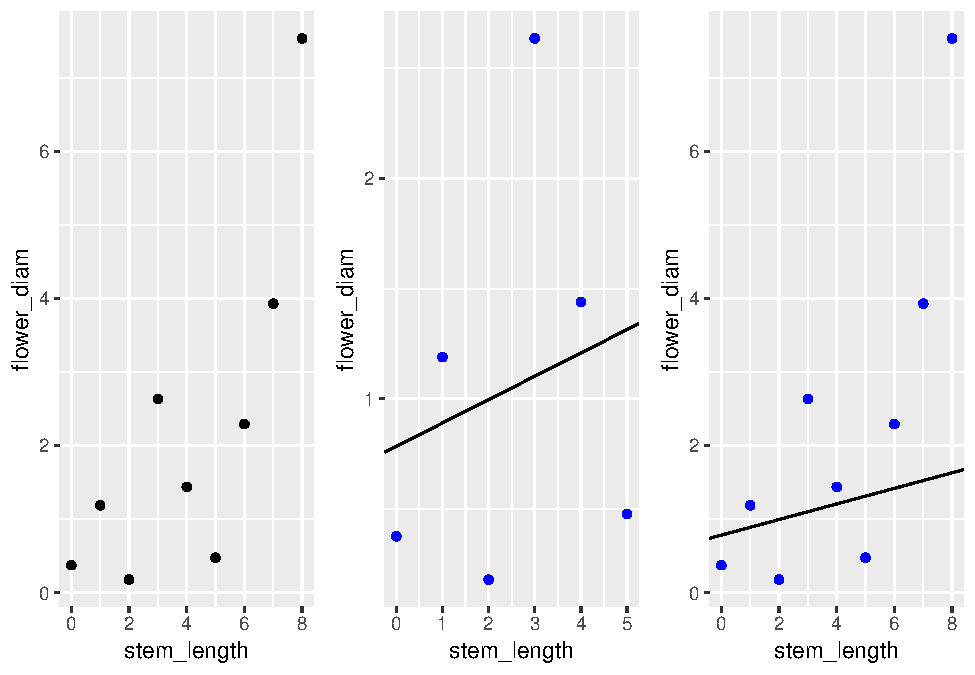
\includegraphics{thesis_files/figure-latex/systematic-1.pdf}

Imputation attempts to address this common dilemma in real-world data.
Imputation is the process of replacing missingness in data sets with
some value that redeems the observation for some degree of analysis.
``The aim of these methods is to compensate for the missing data in such
a manner that the analysis file may be subjected to any form of analysis
without the need for further consideration of the missing data'' (Brick
\& Kalton, 1996). Imputation assigns values to missing responses, which
allows records with missingness to be retained during analysis. Ideally,
imputation would eliminate bias in survey estimates caused by ignoring
records with missing data. The catch is that imputation can destroy
intervariable relationships, as well as overestimate the precision of
survey estimates on fabricated data.

There are stochastic and deterministic methods for imputation.
Deterministic regression imputation is the predicted value from a
regression trained on complete-case data. Stochastic imputation differs
due to an additional residual added term to the predicted value, taken
either from a random respondent or comparable observation, and is
usually preferred due to the importance of shape parameters in many
analyses (Brick \& Kalton, 1996).

One traditional method of imputation is the ``Hot-Deck Method'', which
was generally favorable when computation was less efficient. Hot Deck
Imputation requires extensive knowledge of the survey variables in order
to optimize performance since explicit model-based imputation needs a
valid model for every survey variable (Maiti, Miller, \& Mukhopadhyay,
2008). This thesis proposes naive artificial neural networks as a
solution which requires minimal domain knowledge and resists the curse
of dimensionality which other nonparametric methods are susceptible to,
such as local polynomial regression (Maiti et al., 2008).

Due to the difficulties imposed by working with high-dimensional,
complex survey data with varying degrees of domain knowledge, we turn to
neural networks and their structural benefits to reliably perform these
challenging imputation problems.

\chapter{Neural Networks}\label{math-sci}

\section{Introduction to Machine
Learning}\label{introduction-to-machine-learning}
\begin{quote}
From the advent of computation, there has been a drive towards
automation. (Goodfellow, Bengio, \& Courville, 2016)
\end{quote}
The capacity to derive patterns from raw data is known as machine
learning, a broad term for an extremely diverse collection of
algorithms. Machine learning flips the script on classical programming:
whereas classical programming takes rules and data to produce answers,
machine learning creates rules from data and answers by being ``trained
rather than explicitly programmed. It's presented with many examples
relevant to a task, and it finds a structure that derives rules for
automating the task'' (Chollet \& Allaire, 2018).

Machine learning is intended to elucidate or predict patterns in data.
These algorithms handle anything from linear regression for predicting a
numerical response based on a number of features, to clustering for
visualization and assignment of untaught observation classes. Machine
learning models are trained by minimizing error during exposure to
labelled ``training'' data with some underlying distribution and random
noise. After training, models are passed unlabelled ``test'' data to
predict the corresponding unknown class or value. Predictive
(supervised) machine learning algorithms seek to emulate and elucidate a
true unknown generative function from which the data were drawn.

For imputation purposes, our goal will be to accurately estimate missing
values by approximating the generative function from which they are
drawn. Generative functions are of the form \[
y = f(x_1, x_2, \dots, x_n) + \epsilon
\] where the true label \(y\) of the observation is a function of the
features \(x_1, ..., x_n\) perturbed by some random noise \(\epsilon\).

The estimating model will be trained via exposure to labelled
observations, called the training data, then used to predict
observations with missing labels, called testing data. The challenge in
machine learning is learning the correct amount from training data in
order to derive the underlying distribution of the observations without
simply memorizing the labels of the training set. This memorizaion
problem is called overfitting and is central to machine learning.

\ref{fig:overfit} is an illustration of this pervasive principle in a
regression example. An overfit (or too-flexible) model simply learns the
observation's labels, rather than the underlying distribution (or
generative function, in this case a second-degree polynomial). The
overfit model fails to learn the underlying generative function, and
instead learns the random noise of the training observations, and thus
is a poor explanation of a new realization from the same generative
function, seen in \ref{fig:overfit} and \ref{fig:overfitre}:
\begin{figure}
\centering
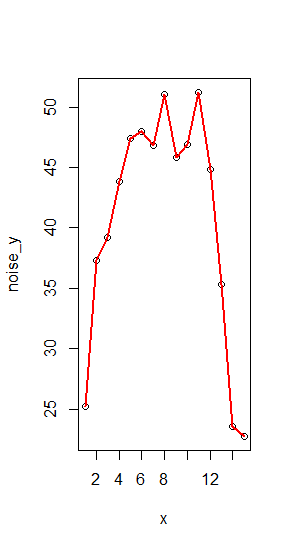
\includegraphics{figure/overfit.png}
\caption{\label{fig:overfit}The overfit model has extremely low error on the
realization of the data on which it was trained.}
\end{figure}
\begin{figure}
\centering
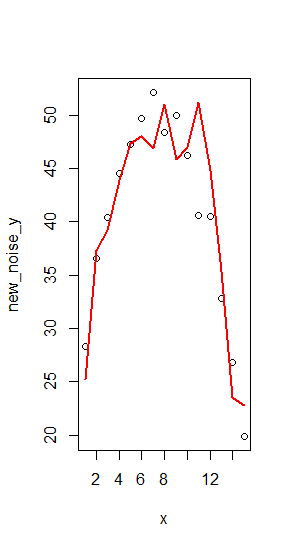
\includegraphics{figure/badfit.png}
\caption{\label{fig:overfitre}The overfit model does not accurately reflect
the underlying distribution from which both datasets are drawn. Rather,
it captures only the random noise of the data on which it was trained.
It would be a mistake to assume the generative function is a degree 15
polynomial just because the training error of such a function is low.}
\end{figure}
An underfit model, \ref{fig:underfit}, also fails to capture the
underlying distribution, due to a lack of flexibility. A linear
regression, though it minimizes its training MSE, clearly fails to
capture the underlying distribution of the data:
\begin{figure}
\centering
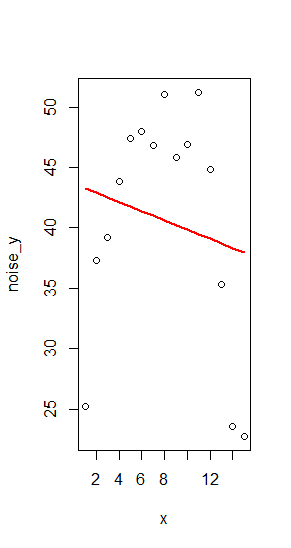
\includegraphics{figure/underfit.png}
\caption{\label{fig:underfit}An underfit model fails to capture the
underlying distribution}
\end{figure}
\ref{fig:underfit} displays a well-trained model which straddles these
extrema and captures the apparent underlying distribution of the data in
a general sense by approximating the generative function from which they
are drawn, and remains fairly constant under different draws from the
same distribution:

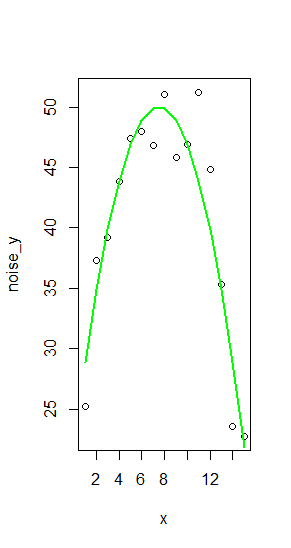
\includegraphics{figure/true.png} 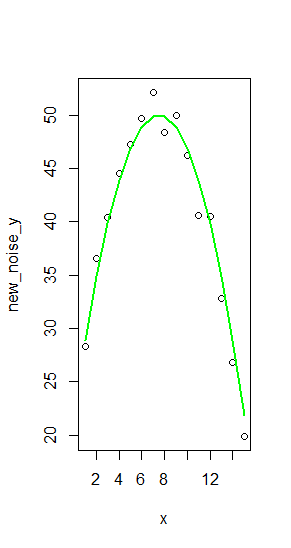
\includegraphics{figure/stayGood.png}
\begin{figure}
\centering
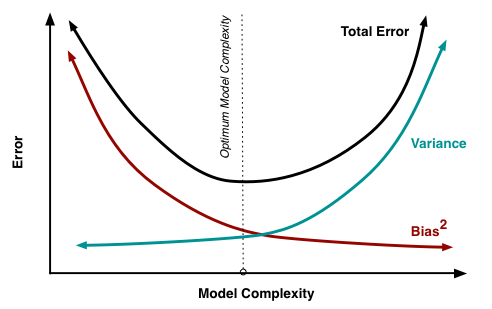
\includegraphics{figure/biasvariance.png}
\caption{\label{fig:biasvar}\url{http://scott.fortmann-roe.com/docs/BiasVariance.html}}
\end{figure}
Fortmann, Scott. ``Bias and Variance.'' Understanding the Bias-Variance
Tradeoff, June 2012, scott.fortmann-roe.com/docs/BiasVariance.html.

Figure \ref{fig:biasvar} demonstrates the involvement of model
complexity (or flexibility) in terms of training error. Model complexity
refers to the ability of the model to approximate complex generative
functions. We see that as the flexibility of the model increases, the
bias on the training set always decreases, representing the model's
performance on observations with labels. However, complexity beyond the
models optimal value implies over-flexibility, in which the model is
able to memorize random noise rather than stopping at the trend of the
data. This increases the total error of the model when exposed to data
that comes from the same generative function that the model has not been
exposed to, such as a testing data set or another observation from
outside the training set. Higher flexibility models create more variable
models, which though trained on data from the same generative function
differ greatly in appearance due to the random sample of training data.
These models are unstable for inference and generalize poorly.

One key difference from statistical modelling and survey statistics
methods is the point at which randomness is introduced into the data.
Machine learning attempts to approximate the function from which the
data was randomly generated, while survey statistics imply that
randomness in data comes from the survey design. The paradox of where
randomness is introduced into the data is resolved with the existence of
a superpopulation \(U\), where each observation has label
\(y = f(x) + \epsilon\), some generative function. From this
superpopulation, a population \(u\) is created through \emph{i.i.d.}
realizations from \(U\). From this population \(u\), the survey is
taken. Thus there still exists a generative function from which the
population is drawn, but the features and label of the observations are
fixed by the time the complex survey is taken on the population,
reconciling the two methodologies.

\section{Neural Networks}\label{neural-networks}

\subsection{Background and Context}\label{background-and-context}

Neural networks are a family of machine learning algorithms with an
extended and diverse history of research in neuroscience, statistics,
and computer science. Recently, these models have experienced great
growth in attention and popularity due to the contemporary circumstance
of computational capability. Neural networks thrive on large training
data sets, which have tended to increase in size and availability
throughout time. Neural networks also outperform competing algorithms in
high-dimension feature problems, which are common in real-world machine
learning applications such as image data, waveform data, and large
surveys. Often utilizing derivatives of complex compositions of
functions as an optimization method, deep learning training periods are
computationally intensive, relying heavily on computer hardware and
optimized software for reasonable implementation. Lastly, recent
attention to and development of neural networks can be attributed to
their proven potential in solving complicated real-world applications
with promising and increasingly dominant accuracy in practice, often at
the cost of a lack of inferability.

This lack of infer-ability is the typical downside of working with
neural networks as the inference on a model can be more important than
the predictive accuracy depending on the problem. Once a simple linear
regression is trained, the coefficients on the predictors offer an
immediately understandable interpretation of the behavior of the data.
For example, a coefficient of .3 on a feature \(x\) has a simple,
instant understanding: as feature \(x\) goes up by 1, the response goes
up by .3. Neural networks however, lack this instant recognition due to
the less intuitive layered structure of input transformations, known as
representation learning.

\subsection{Basics}\label{basics}

Neural Networks are a composition of functions. The following describes
a full neural network:

\[
\hat y = f(x; \theta, \omega) = f^n ( f^{n-1}  ( ... f^1(x)))
\] In this function, we see the input features \(x\), the learned
coefficients \(\theta\), the learning rate \(\omega\), and the output
prediction \(\hat{y}\). Consider one of the layers of the network,
\(f_i\). This layer is an activation function on linear function:

\[
f^i = \max ( 0 , {W_i}^T x + c_i)
\]

The activation function shown above is the rectified linear unit, or
\(\max(0,a)\). Activation functions are significant as they introduce
nonlinearity into what would otherwise be a linear function (a
composition of linear functions). \({W_i}^T\) and \(c\) in \(f_i\)
dictate a linear transformation on the input to the layer. An ordered
list of all elements of \(W_i\) and \(c_i\) for all \(i \in n\) would
give the full description of the network, called \(\theta\). So the
output of a 1-layer network can be expressed as

\[
f(x; W, c, w, b) = w^T \max( 0 , W^T x +c ) +b
\]

The final activation function is another structural parameter left to
the designer of the network. The typical choices are
\begin{enumerate}
\def\labelenumi{\arabic{enumi}.}
\tightlist
\item
  Linear units for Gaussian output distributions
\item
  Sigmoid units for Bernoulli output distributions
\item
  Softmax units for Multinoulli output distributions
\end{enumerate}
(Goodfellow et al., 2016)

The learning rate \(\omega\) and a loss function are meta-parameters,
given by the user creating the neural network. These two parameters are
used during the training of the network. During training, gradient
descent is used to descend the loss function in order to find the
optimal parameters for the network.

Loss functions are ways of describing performance of a model when
predicting labels of a data set. The loss function takes the model and
data as inputs, and outputs a real number. Loss functions can be
minimized in training by optimization which leads the network to find
improvements in weights yielding accurate predictions. Loss functions
allow for another degree of customization in the training of a network,
such as in Ridge and LASSO regression. These algorithms add a weighting
to the typical mean squared error loss function which penalizes the
weights on predictors in polynomial regression. These methods introduce
bias into otherwise unbiased algorithms, but reduce the variability of
the model across different draws of data from the same distribution,
aiming to reduce the real test loss and improve the model. The cross
entropy between the data distribution and the model distribution is the
typical choice (Goodfellow et al., 2016).

Cross Entropy: \[
\int_\chi P(x) \log Q (x) dr(x) = E_p [- \log Q]
\]

Take for example the Mean Squared Error cost function: \[
MSE = \frac{1}{n} \sum_{k=1}^n  (y - \hat y)
\]

MSE, a typical loss function for regression applications, takes the mean
squared difference of the predicted label \(\hat y\) and the true label
\(y\) of the observations.
\begin{figure}
\centering
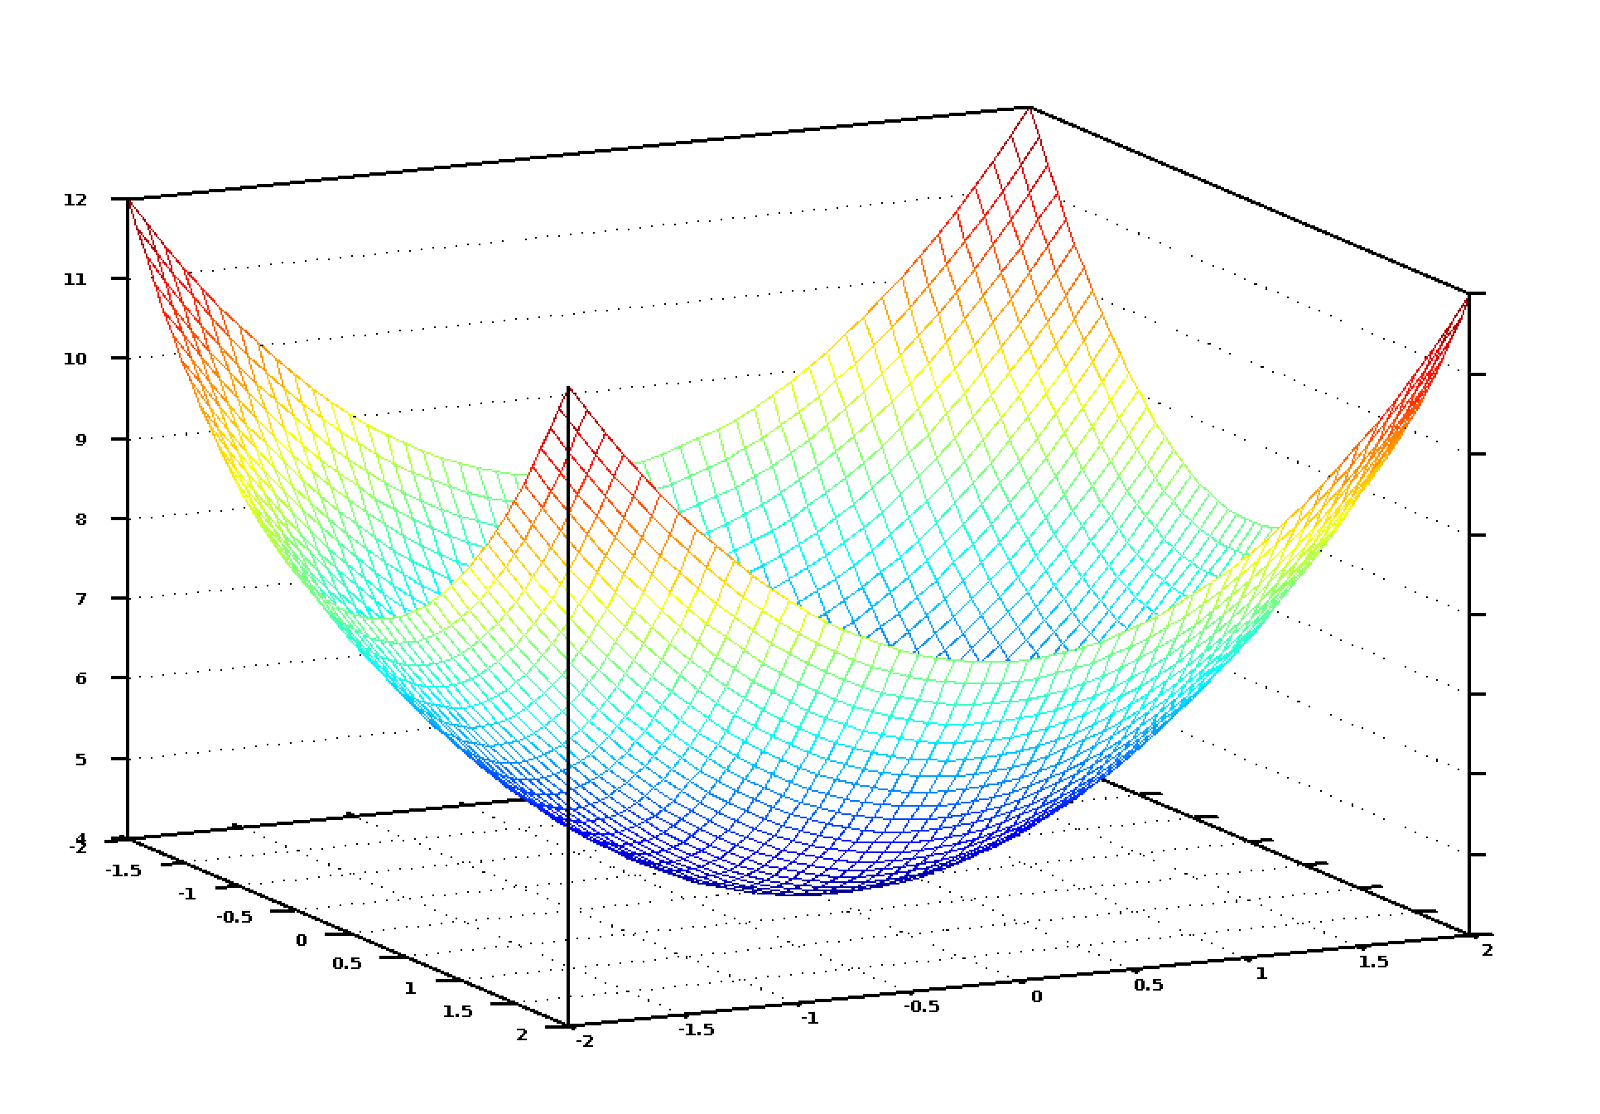
\includegraphics{figure/optimize.png}
\caption{\label{fig:optimize}\url{https://medium.com/@ageitgey/machine-learning-is-fun-80ea3ec3c471}}
\end{figure}
Can improve this image and example, but the lesson is good.

Figure \ref{fig:optimize}

We can see that the loss of a linear regression is a function of \(m\)
and \(c\) given some data which is minimized at \(m = 0\) and \(c = 0\).
The learning rate is the amount that the functions' coefficients are
updated as the loss function is optimized.

Much like training a linear regression, the training of the neural
network aims to drive the approximating function to the underlying
function. The important difference induced by nonparametric models,
however, is the nonconvexity of the loss. The large amount of
coefficients which define even a relatively small network complicate the
optimization problem and make local minima a demanding distraction.
Optimization is typically done with gradient learning using a loss
function, or maximum likelihood estimation. Most modern neural networks
are trained using maximum likelihood, in which the cost function is the
negative log-likelihood between the training data and model distribution
(Goodfellow et al., 2016).

\subsection{Representation Learning}\label{representation-learning}

{[}{[}kelly, tell me if i should just delete this cheesy
paragraph:{]}{]} If you were handed a photograph and were asked if it
contained a car, there's a good chance you would immediately know the
answer. But how are you coming to this conclusion? The human mind
recognizes patterns of the image it has seen before, like a round
bumper, a rectangular windshield, and a few circular tires with a
certain spatial relationship to come to the conclusion that there is, in
fact, a car in the photograph. It is this process of representation
learning that prompted early researchers {[}{[}Citation Needed{]}{]} to
create representation-based learning algorithms to extrapolate on
information in the same way as the human mind. The emulation of human
neural cells was the birth of deep learning, a class of machine learning
algorithms which takes its name from multiple layers of connected nodes
simulating a proposed structure of the neurons of the human mind.
Representation learning takes observation's features as a first layer
into a composition of functions, in which each layer (or function)
transforms the data according to a learned representation transformation
that the subsequent layer takes as an input. This composition allows for
complex relationships of features to be learned in increasingly
sophisticated ways, making neural networks ideal for large-dimensional
datasets. For large-dimensional features, such as in Consumer Spending
Data, images, or audio, these hierarchical representations (or layered
representations) are important for distilling human-like feature
extraction and iterative predictor space transformation. To achieve
hierarchical representation properties, subsequent layers understand
more complex functions of input variables as each layer transforms
inputs and optimizes weights and weight relationships that minimize the
overall loss of the network. As each layer receives the transformed
output of the previous layer, more complex relationships of features can
be derived.

Successive layers of the network learn representation transformations of
the data which lend themselves to increasingly accurate description by
linear regression and activation performed by the final layer, called
the output layer. This process of successive transformation learns
meaningful representations on which the output layer can be most
accurate. Since the full network does not have a single functional
representation, it is nonparametric. The flexibility and power of neural
networks in fields demanding domain knowledge is that they can
approximate any function, per the Universal Approximation Theorem
(Hornik et al., 1989; Cybenko, 1989). The theorem states that a
feedforward network with a linear output layer and at least one hidden
layer with any ``squashing'' activation function can approximate any
Borel measurable function from one finite-dimensional space to another
with any desired nonzero amount of error, provided that the network is
given enough hidden units. Thus the user decision required is the depth
and breadth of the network, optimized through validation set
meta-analysis.

Representation learning is extremely important to the broad promises of
neural networks in practice. The basis for this strength is that
subsequent layers of the network learn meaningful structures of the
input data associated with a lower loss score. Correlations of features
forming a functional relationship to the label which induce loss
function descent will be internalized by the composition of subsequent
functions. This property of representation learning is significant for
investigating the necessity of independent and identically distributed
data in deep learning algorithms. It could be the case that the
significance of the inclusion probability can be learned as a meaningful
feature, with no special tweaks or preprocessing necessary for the
algorithm. Data which require no special tweeks are extremely meaningful
as this circumvents the necessity of incorporating domain knowledge and
expertise in current imputation methods, which holds back expedient and
lightweight research.

These advantages of Hierarchical and Distributed Representation
transformation give neural networks huge advantages in accuracy and
fitting capability for data with a massive hypothesis space. A
hypothesis space is the space of all possible answers to a question.
Image classification, for instance, represents a hypothesis space of
pixels with unknown correlations that must be trained with label
relationships to determine the correct distillation of millions of
pixels to a most-likely class label. Thus the curse of dimensionality
common throughout machine learning is mitigated through this manifold
learning process.

Neural networks thrive on the interaction of many features, due to the
nature of representation learning which excels in covariate relations
and distilling information encoded between features. Popular modern
applications are image and waveform audio data, in which machine
learning problems become dominated by the Curse of Dimensionality. This
common machine learning problem arises when the amount of data is
insignificant when compared to the hypothesis space or feature space,
and there are sparse observations for some regions. Machine learning
needs many observations with each combination of values, but this
becomes quickly infeasible for data with thousands of features. The
peaking phenomena dictates that there is an optimal number of features
to describe the data before the curse of dimensionality creates
problematic sparsity and dominating observations with few neighbors .
Neural networks are known to resist this commonplace issue due to the
distributed learning property, wherein each node is sensitive to only
particular features.

Distributed representation is a powerful implicit component of neural
networks in which neurons divide feature space to better handle feature
interactions: suppose an image-recognition system could recognize cars,
trucks, and birds, as well as distinguish if these objects are red,
green, or blue. One way of representing these inputs could be to have a
separate neuron for each combination: red truck, red car, red bird, and
so on for nine independent neurons. Distributed representation, however,
could partition these workloads by having three neurons for color and
three for object type. In addition to reducing the number of neurons
required dimensionally, this also distributes the learning demands of
each neuron. The neuron describing redness is able to learn about
redness from any category, not one specific category as the red bird
neuron must (Goodfellow et al., 2016).

Neural networks approximate nonlinear functions by applying linear
models not to the features x, but to a transformed input, \(\phi(x)\),
where \(\phi\) is a nonlinear transformation. \(\phi\) provides a new,
more meaningful representation for \(x\). The question then is how to
choose the mapping \(\phi\):
\begin{enumerate}
\def\labelenumi{\arabic{enumi}.}
\item
  One option is to manually engineer \(\phi\). This takes a huge
  speciality of domain knowledge and practitioner specialization, with
  little transfer between domains. This was the dominant method before
  deep learning (Goodfellow et al., 2016).
\item
  The strategy of neural networks comes from the learning of \(\phi\).
  ``In this approach, we have a model y = f(x; theta, w) as specified in
  the neural network introduction. Due to the Universal Approximation
  Theorem, the nonparametric deep feedforward network can learn a
  functional approximation from the input to the desired output. This
  method sacrifices the training convexity of the other two, but
  benefits from the genericity of the specifications. The human user
  need only specify a general function family rather than exactly the
  correct function, but can still benefit from designing families of
  \(\phi(x; \theta)\) that they expect to be relevant (Goodfellow et
  al., 2016).
\end{enumerate}
The neural network approximates some true underlying function
\(f^*(p; \theta)\) of the predictors \(x\) to the output category,
\(y\), and learns the coefficients \(\theta\) of the series of linear
transformations composing the layers that result in the best function
approximation. The number of functions in the composition is the called
the depth of the model. Our model is called \(\hat f\), the generative
function it seeks to approximate is called \(f\). The outputs of our
model are \(\hat y\) ``guess at y'' and the true labels are \(y\).

\subsection{Neural Networks for Complex Survey
Data}\label{neural-networks-for-complex-survey-data}

From an optimist's perspective, the need for data preprocessing or
special conditions on the loss function for training the model would be
unnecessary: If learning the correlations and underlying distributions
associated with rare observations from complex survey design would truly
lower the network's loss, it should be learned and accounted for without
the need to perform special external transformations on the data to
``undo'' the effects of complex sample design. For this reason, it is
significant to compare the potentially superior results of a naive model
to one with superfluous data transformations done. A neural network
model with access to an informative \(\pi\) feature ideally would
approximate the function relating the inclusion probability and features
to labels, without the need for extreme domain knowledge and manual
feature engineering.

The optimism of nonparametric algorithms increases in tasks of minimal
domain knowledge and feature engineering capability. Ideally, using
heuristic meta-parameters defining a neural network model would be
enough to get reasonable predictive accuracy in conjunction with one of
the methods of Chapter 3. Per the Universal Approximation Theorem, any
underlying generative function is at worst approximated by a 2 layer
heuristic model, potentially improving upon other naive modeling
procedures such as a weighted linear regression. Additionally, in real
survey data the capacity to derive the significant features from a
high-dimensional space is a weakness of parametric model regression,
which is highly variable in the context of noisy parameters, explored in
Chapter 4.

\chapter{Methods}\label{methods}

Missingness is an extremely common problem in real data sets. Many
analyses and algorithms such as regression, classification, PCA, and
clustering done throughout the sciences rely on having entirely complete
observations. For this reason, some strategy must be adopted to
transform a raw data set into an analyzable one.

There are multiple approaches for a researcher interested in going about
this process. The researcher has a data set gathered under a complex
survey design where the features \(x_1,...x_n\) and inclusion
probability \(\pi_i\) is known for all \(i\), though the label \(y_i\)
may be missing due to item nonresponse. In order to create a data set
with no missing values, the researcher may choose to adopt one of the
following methods. These methods borrow notions from complex survey
design about using design variables to model how characteristics of the
population affecting the sample (Maiti et al., 2008). Neural network
methods have the advantage of flexibility in approximating any
functional relationship, and can be tuned using sampling weights to
account for complex sampling design using unequal sampling (Maiti et
al., 2008).

There are two primary tasks for a researcher: representative
complete-case data, and statistic estimation via accurate imputation.
The following methods are imputation techniques designed with these
goals in mind. Imputation methods utilize different techniques to create
a complete-case dataset by estimating missing values based on
information from the complete cases. Once the missing values are
imputed, the population statistic is estimated and the approximate
complete-case data set may be used.

\section{Mean Estimation Methods}\label{mean-estimation-methods}

A common statistic of interest to a researcher is an estimate of the
population mean \(\mu_y\) using the information from the complex sample
with missingness, but taking the naive mean of complete cases is
insufficient for two reasons. The first has been discussed in Chapter 1,
which is the potential of systematic missingness in the data. The second
is that the naive mean makes the assumption that the observations
represent equal proportions of the population, as in an \emph{i.i.d.}
sample.

Naive Mean: \[
\hat \mu_y = \frac{1}{r} \sum_{i=1}^r y_i
\] Where \(r\) are the complete-case respondents.

We resolve this issue in the mean estimate formula by weighting
contributions to the mean by \(\frac{1}{\pi_i}\), the approximate number
of population members represented by observation \(i\):

\subsection{Pi-Corrected Naive Mean:}\label{pi-corrected-naive-mean}

\[
\hat \mu_y = \frac{1}{\hat N} \sum_{i=1}^r y_i \frac{1}{\pi_i}
\] Where \(\hat N = \sum_{i=1}^r \frac{1}{\pi_i}\). This resolves the
problem of ignoring the survey design in estimation, but does not
account for systematic bias resulting from missingness. This will be an
under-estimate of the true population mean in the presence of systematic
missingess of large observations.

Let \(\hat \mu_y\) be the sample estimate of the population mean
\(\mu_y\). The oracle mean can be considered the ``best estimate'' of
\(\mu_y\), but it is only available in simulation. The oracle mean uses
information that the simulation manually drops so as to create an ideal
population estimate given a survey sample:

\subsection{Oracle Mean:}\label{oracle-mean}

\[
\hat \mu_{\text{oracle}} = \frac{1}{n} \sum_{i=1}^n y_i \frac{1}{\pi_i}
\] The oracle mean will be used as a benchmark against which the other
methods will be compared.

In order to combat the presence of systematic missing values, we utilize
imputation to label the missing observations with the best estimate of
\(y_i\), \(\hat y_i\). Imputation has the added benefit of approximating
a complete-case dataset without dropping observations.

\subsection{Imputation Mean Estimator:}\label{imputation-mean-estimator}

\[
\hat \mu_y(\text{method}) = \frac{1}{\hat N} (\sum_{i=1}^{r} \frac{y_i}{\pi_i} + \sum_{i=1}^{y-r} \frac{\hat y_i}{\pi_i})
\] Where \(y-r\) are the missing cases, \(r\) are the respondents, and
\(\hat N = \sum_{i=1}^n \frac{1}{\pi_i}\).

\subsection{Drop.NA}\label{drop.na}

One option is to simply remove the observations with missing labels from
the data set. This method is extremely easy to implement and serves as a
sure-fire way to end up with a data set with no missing values. There
are two downsides to this method: The first is that removing
observations with missingness obviously decreases the size of the data
set and can nontrivially reduce the fidelity of models aiming to
understand the population from which the data was taken. The second
problem is the assumption of random missingness. If there is any
correlation of label to amount of missingness, systematic bias is
introduced into the data set, as discussed in Chapter 1. For example, if
there is a possibility that larger values are more likely to be dropped,
then as a result the sample mean would underestimate the population
mean.

\subsection{Median Imputation}\label{median-imputation}

Median imputation is another easy way to get complete cases in data for
analysis or estimation. Median imputation simply fills in the missing
labels with the median of the respondent labels. Median imputation has
multiple problems for analysis or estimation. The median offers equal
weighting to all observations in a data set, meaning it destroys the
informativity of the inclusion probability \(\pi\). It also removes
correlation of feature and label, making analyses such as PCA less
informative, as covariate relations dictate axis derivations. Median
imputation is extremely fast to execute and implement, but creates
noninformative observations in the same manner as the Drop.NA method.

\subsection{Linear Regression Imputation (weighted
pi)}\label{linear-regression-imputation-weighted-pi}

Linear regression is a convex optimization problem of \(n+1\)
parameters, where \(\hat f(x) = \hat y = (m_1x_1 + .+ m_nx_n)+b\) is the
estimate of \(y\) for observation \(i\). Using the mean of the squared
difference between the predicted and actual responses of a training data
set, Weighted-MSE Linear Regression scales the squared error
contribution of each observation by \(\frac{1}{\pi_i}\) to account for
rare-case observations with potentially systematic missingess: \[
\text{MSE}(f) = \frac{1}{r} \sum_{i=1}^r  (\frac{1}{\pi}(\hat{y} - y))^2
\]

\subsection{Naive Neural Network
Imputation}\label{naive-neural-network-imputation}

Neural Network Imputation is our baseline model for imputation for
estimating a population mean. The number of hidden layers, nodes, and
loss is left to the user, which would be an incorporation of domain
knowledge or exploratory modelling to derive a reasonable model load for
learning the data's generative function. In the context of the
researcher having minimal knowledge of the data, a neural network with 2
hidden layers of 32 units activated by \texttt{relu} functions is a
reasonable starting point. Overtraining due to overflexible models can
be stimied with a validation set, assuming the data is not small
(\(n > 10^3\)). ``Naive'' neural network imputation refers to this model
not having access to the \(\pi\) feature of the observations as a
predictor or incorporate it in any way. This model uses the assumption
that the data is \emph{i.i.d} as a representative for ignoring the
survey design, an assumption which is known to be a significant problem.
Regardless, the neural network should approximate the generative
function with some nonparametric fit, but underestimate the population
mean as a result of systematic missingness and observation equity.

\subsection{Loss-Weighted Neural Network
Imputation}\label{loss-weighted-neural-network-imputation}

Loss-Weighted Neural Network Imputation takes inspiration from the
weighted linear regression algorithm. This neural network training uses
the same \(\pi\)-weighted MSE, but sacrifices the convexity of the loss
function, which means pervasive local minima which are distracting to
the learning algorithm. The existence of local minima from the
high-dimensional model space comes from the flexibility of the many
hidden neurons weight transformations within the model. A loss-weighted
neural network hopes to account for systematic missingness in the data
by heavily punishing the loss term generated from rarer observations.
Since rare observations are more likely to be missing, they must be
given more weight since they appear less in the training data then the
population. Thus a weighting scheme attempts to un-do systematic
missingness by making the rarer observations as ``heavy'' as they would
be in the true population by making outliers be worth multiple
observations to the loss contribution.

\subsection{\texorpdfstring{\(\pi\)-Feature Neural Network
Imputation}{\textbackslash{}pi-Feature Neural Network Imputation}}\label{pi-feature-neural-network-imputation}

A \(\pi\)-feature neural network has access to \(\pi\) as a predictor
during training and testing. This is a realistic assumption to make as
data collected under a complex survey design must have a \(\pi\)
probability regardless of whether the label is missing. This method has
the benefit of adapting to whether \(\pi\) is truly correlated to \(y\),
which the loss-weighted method assumes. A neural network optimist could
claim that if there is a significant relationship of \(\pi\) to \(y\),
it will be reflected in the loss during training and the network will
adapt accordingly to the information provided by the feature. However if
\(\pi\) and \(y\) are uncorrelated and the missingess is random, the
network will not still weight the observations and will correctly ignore
the feature to create more accurate predictions with no need for domain
knowledge on the relationship of the missingness.

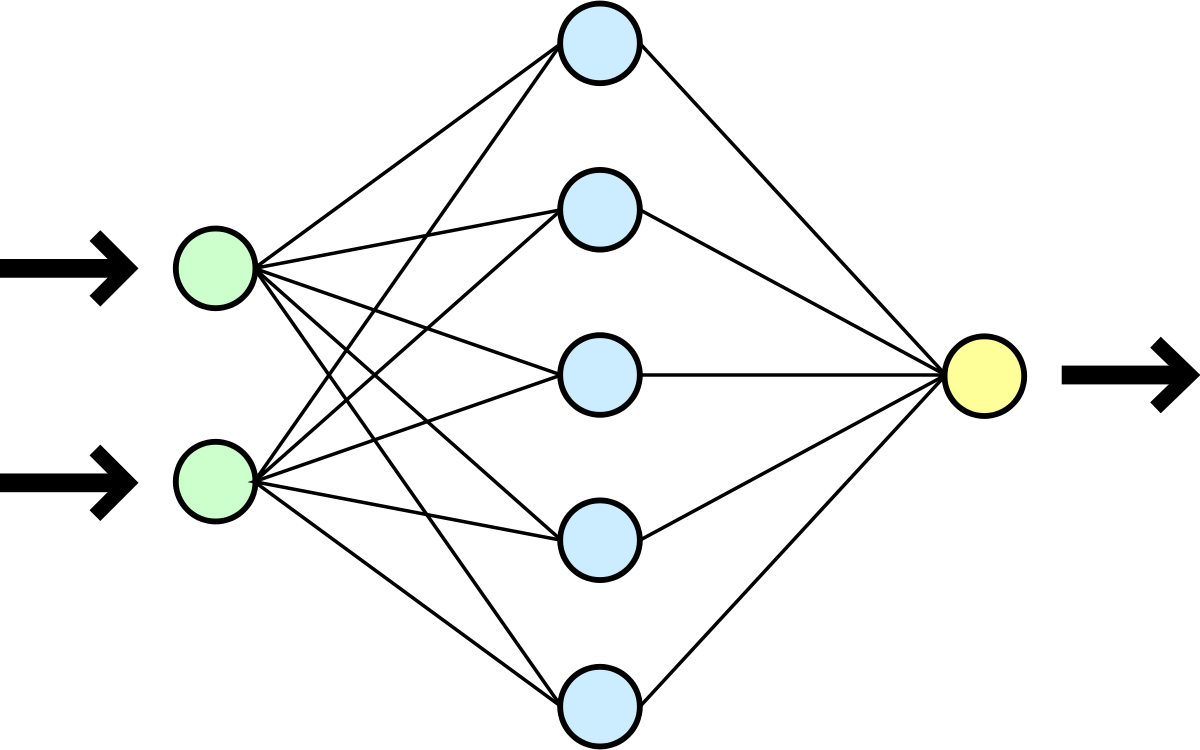
\includegraphics{figure/network.png}

\subsection{Weighted Resample Neural Network
Imputation}\label{weighted-resample-neural-network-imputation}

The weighted resample method uses the same model as the naive neural
network imputation but uses a data preprocessing step to incorporate the
survey design information. A weighted resample of size \(n\) is taken
from the sample with replacement with observation selected by
probability \(\frac{1}{\pi}\). The inference of this method is an
attempt to ``undo'' the effects of survey design in gathering the data.
A weighted resample in which observations are selected by the inverse
inclusion probability uses the insight that an observation with
inclusion probability \(\pi\) represents \(\frac{1}{\pi}\) members of
the population. By sampling on this probability, the resampled data set
should be an estimate of an \emph{i.i.d.} sample from the population,
making it viable for supervised learning ignoring the survey design
elements. From this point the naive neural network method is applied
(and directly compared to naive neural network estimates), since ideally
this is \emph{i.i.d} data without need for survey design information
tweaks on the algorithm.

\subsection{Derived Feature Neural Network
Imputation}\label{derived-feature-neural-network-imputation}

This method pre-processes the data by deriving additional features, such
as the product of two features and the product of a feature and the
inclusion probability. The intention of this method is expediting the
training process to allow the approximation of more complex generative
functions with less model capacity and training. Intuitively, the
relationship of \(\pi\) to \(x_i\) in the missing data, should it be
relevant, will be more easily learned for superior prediction accuracy.

\chapter{Simulation}\label{simulation}

\section{Exploration of Methods Using
Simulation}\label{exploration-of-methods-using-simulation}

Simulated data is used to evaluate the methods in order to get an
understanding of their performance on a data set with known
characteristics.

Full insight into the feature distributions, generative function, random
noise, and systematic missingness allow for controlled experimentation
on when certain methods thrive. Simulation allows for parameters such as
label noise and feature informativity to be changed and measure the
response of the methods across any domain.

\section{High-Dimension Simulation}\label{high-dimension-simulation}

Often in real-world data, there might be a large number of features, not
all of which are necessarily correlated to the response label. For
example in the Consumer Expenditure data, age, gender, ethnicity, and
education might have a predictive relationship with income, while a
number of others such as XXXXXXX do not. The ability for a model to
discern which features are relevant and which are not is a significant
benefit both for inference and predictive consistency. Inspired by
research in best feature selection methods, non-correlated features are
used in the model evaluation step in an attempt to more realistically
simulate complex data (Hastie, Tibshirani, \& Tibshirani, 2017). The
addition of these features contributes to the curse of dimensionality
and variability of estimates.

These additional ``noisy'' parameters are simulated by making the
generative function of the labels \(y\) not a function of some of the
features. All methods used in the simulation are accompanied by their
oracle counterparts, meaning the same method is run two times: one with
access to all features, the oracle restricted only to the relevant
features which are inputs to the generative function.

\section{Monte Carlo Simulation}\label{monte-carlo-simulation}

Monte Carlo (MC) simulation attempts to overcome the inherent randomness
of sampling and model training by repeated iterations of the sampling,
training, and evaluation steps. A distribution of output estimates is
made over many potential samples from the population in order to get a
more complete interpretation of the results.

It should be noted that neural networks can be more optimized than in
their performance in the following simulation study. This is because a
network can be intentionally over-trained on the training data, then
re-trained from scratch to the number of epochs which minimized the
validation loss. This poses a challenge in MC simulation, however, where
many iterations without user input are needed. Additionally, runtime
becomes a vastly greater concern when networks must be over-trained
through many epochs, more than doubling the execution time. If
computation were no expense, the neural network methods could be
expected to be more accurate than the below results.

\section{Creating a Simulated
Population}\label{creating-a-simulated-population}

The size of the population is \(N=10^5\) and the sample is \(n=10^3\)
observations. Despite neural networks thriving in higher-dimension
settings (both of features and observations), complex surveys are often
implemented on real data with scarce observations, making a lower-size
simulation more suitable for generalizability.

The features simulated population is made as the first step of the
process. Two informative features \(p_1, p_2\) are drawn from random
uniform distribution: \[
f(x) = \frac{1}{30+30} \text{ for } x \in (-30, 30)
\] In addition to two informative features, there are \(20\)
uninformative features drawn from the normal distribution. This
distribution is arbitrary but can have unintended consequences due to
accidental correlation, noted in \{Hastie et al. (2017)\}.

The population labels \(y\) are a nonlinear function of the informative
features: \[
y = p_1^2 + p_2^2
\] The labels are then made nonpolynomial by contorting the parabola
into a ``bowl with flat lip'': \[
y' = \left\{ \begin{array}{cc} 
                y & \hspace{5mm} y<\bar{y} \\
                \bar{y} & \hspace{5mm} y \geq \bar{y} \\
                \end{array} \right.
\]

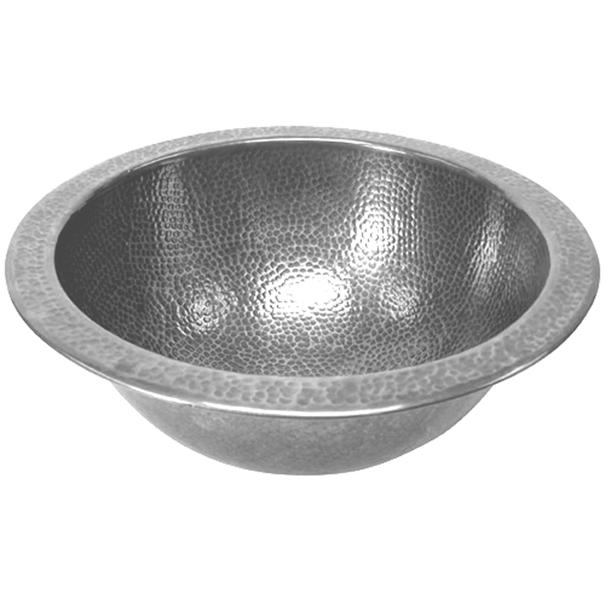
\includegraphics{figure/bowl.jpg}

Random noise \(\epsilon\) with \(\sigma = 1\) is then added to the
transformed labels: \[
y'' = y' + \epsilon_y
\]

An inclusion probability \(pi\) is then assigned to each observation
with a strong correlation to \(y\), as well as random normal noise with
\(\sigma = 1\): \[
\pi = \sqrt{y''} + \epsilon_\pi
\] These values are then rescaled to (0,1) and rescaled so
\(\sum_i^N \pi_i = n\).

Combining the information \(y,\pi, p_1, p_2\) and uncorrelated features
gives the population on which the simulation will be performed. The true
mean of the population labels \(\mu_y\) is now known and recorded.

The Monte Carlo simulation is performed for 100 iterations. This is a
low number of trials, but is constrained by the computation intensity of
running 10 neural networks trained for hundreds of iterations each, as
well as performing many weighted samples.

Within each iteration, a single estimation procedure is performed.
First, a weighted sample from the population is taken with respect to
the inclusion probabilities \(\pi_i\) on each observation. From this
sample of \(n=10^3\) observations, an oracle data set is made by
dropping the noise columns, keeping only \(p_1, p_2, \pi,\) and \(y\).
This data set will be used as a benchmark to mirror each imputation
method in order to gauge the potentially harmful effects of
uninformative features common to real data.

The first step is to record the oracle mean, calculated using
information the other methods are not privy to: \[
\hat \mu_{\text{oracle}} = \frac{1}{n} \sum_{i=1}^n y_i \frac{1}{\pi_i}
\]

All subsequent methods are the methods of study, to be performed where
there is missingness in the data. \(20\%\) of the observations manually
have their labels dropped weighted by \(y\), so large labels are more
likely to be absent. The result is the form of data we are using to
simulate method performance: a complex sample taken from a population
with some kind of systematic bias in item response.

The \(\pi\)-corrected mean estimate, weighted linear regression, and
median imputation methods are all described fully in chapter 3, and are
closed-form algorithms with no randomness in the fitting and estimation
processes. The neural network models, however, have a much larger degree
of flexibility and randomness involved in the implementation and
execution of the estimate during simulation making monte carlo
variability more pronounced.

Neural networks are trained using normalized data on non-convex loss
curves in high-dimensional space, making their optimization process
stochastic. This simulation uses the heuristic \texttt{adam} optimizer.
Each model in this simulation uses a 2 hidden layer network with 32
hidden units per layer to make results and applications more comparable.
Each layer is wrapped in the \texttt{relu} activation function: \[
\text{relu}(x) = \max(0,x)
\] The breadth and depth used here is a heuristic size which could
potentially be optimized to suit the problem. This, however, creates a
conflict of interest with information leakage which the other methods
are not privy to, which induces bias for the success of these
algorithms. To maintain the narrative of a minimal-knowledge naive fit,
these models use a reasonable exploratory capacity. The models in the
fitting process are manually over-trained, then re-trained from scratch
to an optimal state. This is done using a validation data set of
\(15\%\) of the training data. Once trained to an approximate loss
minima, the models predict on holdout test data (the observations
missing labels) and the population mean estimate is computed and
recorded.

\section{Results aaaaaaaaa}\label{results-aaaaaaaaa}

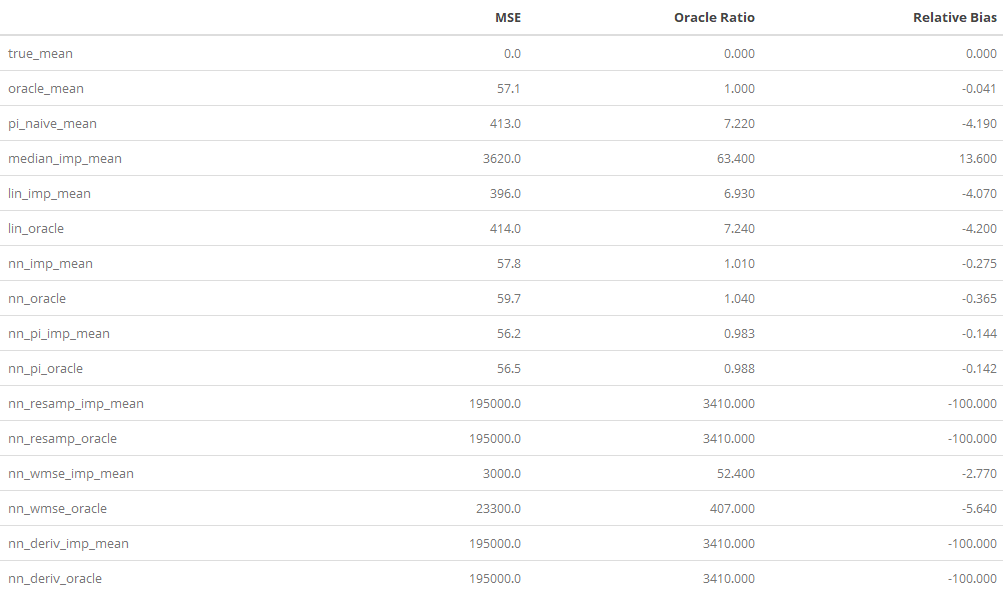
\includegraphics{figure/newresults.png}

Note to Kelly reviewing this: the resampling method and derived
parameters method were left out of this for runtime concerns. I think I
have to find some way to cloud-compute to be able to do some 100+
iterations with all the methods.

I'm hesitant to write too much about results given the situation.

\chapter{realdata aaaaaaaaaa}\label{realdata-aaaaaaaaaa}

aaaaaaaaaaaaaaa

\chapter*{Conclusion}\label{conclusion}
\addcontentsline{toc}{chapter}{Conclusion}

If we don't want Conclusion to have a chapter number next to it, we can
add the \texttt{\{-\}} attribute.

\textbf{More info}

And here's some other random info: the first paragraph after a chapter
title or section head \emph{shouldn't be} indented, because indents are
to tell the reader that you're starting a new paragraph. Since that's
obvious after a chapter or section title, proper typesetting doesn't add
an indent there.

\section{Future Work}\label{future-work}

There are so many exciting unexplored methods and tweaks that would be
worth investigating.

Many I don't know how to implement, couldn't find a good use, don't
understand enough, or was computationally restricted, especially during
monte carlo simulation!

Can do a paragraph on the most important things here:
\begin{itemize}
\tightlist
\item
  something better than linear regression: local polynomial, etc
\item
  training neural networks correctly: finding the validation minima then
  re-training every time. I was prevented by computational intensity
\item
  tweaks on neural networks: \textbf{reinforcement learning}, dropout
  layers, noise layers, pre-trained networks
\item
  re-visiting weighted resampling by trying bootstrapping methods,
  bigger resample. bootstrapping many datasets, training on each, and
  taking mean of estimates. somethign like this to stabilize predictions
  and sampling variability.
\end{itemize}
Multiple imputation: since hopefully NN preserve intervarabhle
relationships better than linear or median etc

\appendix

\chapter{The First Appendix}\label{the-first-appendix}

This first appendix includes all of the R chunks of code that were
hidden throughout the document (using the \texttt{include\ =\ FALSE}
chunk tag) to help with readibility and/or setup.

\textbf{In the main Rmd file}
\begin{Shaded}
\begin{Highlighting}[]
\CommentTok{# This chunk ensures that the thesisdown package is}
\CommentTok{# installed and loaded. This thesisdown package includes}
\CommentTok{# the template files for the thesis.}
\ControlFlowTok{if}\NormalTok{(}\OperatorTok{!}\KeywordTok{require}\NormalTok{(devtools))}
  \KeywordTok{install.packages}\NormalTok{(}\StringTok{"devtools"}\NormalTok{, }\DataTypeTok{repos =} \StringTok{"http://cran.rstudio.com"}\NormalTok{)}
\ControlFlowTok{if}\NormalTok{(}\OperatorTok{!}\KeywordTok{require}\NormalTok{(thesisdown))}
\NormalTok{  devtools}\OperatorTok{::}\KeywordTok{install_github}\NormalTok{(}\StringTok{"ismayc/thesisdown"}\NormalTok{)}
\KeywordTok{library}\NormalTok{(thesisdown)}
\end{Highlighting}
\end{Shaded}
\textbf{In Chapter \ref{ref-labels}:}

\chapter{The Second Appendix, for
Fun}\label{the-second-appendix-for-fun}

\backmatter

\chapter*{References}\label{references}
\addcontentsline{toc}{chapter}{References}

\markboth{References}{References}

\noindent

\setlength{\parindent}{-0.20in} \setlength{\leftskip}{0.20in}
\setlength{\parskip}{8pt}

\hypertarget{refs}{}
\hypertarget{ref-angel2000}{}
Angel, E. (2000). \emph{Interactive computer graphics : A top-down
approach with opengl}. Boston, MA: Addison Wesley Longman.

\hypertarget{ref-angel2001}{}
Angel, E. (2001a). \emph{Batch-file computer graphics : A bottom-up
approach with quicktime}. Boston, MA: Wesley Addison Longman.

\hypertarget{ref-angel2002a}{}
Angel, E. (2001b). \emph{Test second book by angel}. Boston, MA: Wesley
Addison Longman.

\hypertarget{ref-brick1996handling}{}
Brick, J. M., \& Kalton, G. (1996). Handling missing data in survey
research. \emph{Statistical Methods in Medical Research}, \emph{5}(3),
215--238.

\hypertarget{ref-chollet2018deep}{}
Chollet, F., \& Allaire, J. (2018). Deep learning with r. manning
publications.

\hypertarget{ref-goodfellow2016deep}{}
Goodfellow, I., Bengio, Y., \& Courville, A. (2016). \emph{Deep
learning}. MIT press.

\hypertarget{ref-hastie2017extended}{}
Hastie, T., Tibshirani, R., \& Tibshirani, R. J. (2017). Extended
comparisons of best subset selection, forward stepwise selection, and
the lasso. \emph{arXiv Preprint arXiv:1707.08692}.

\hypertarget{ref-lumley2011complex}{}
Lumley, T. (2011). \emph{Complex surveys: A guide to analysis using r}
(Vol. 565). John Wiley \& Sons.

\hypertarget{ref-maiti2008neural}{}
Maiti, T., Miller, C. P., \& Mukhopadhyay, P. K. (2008). Neural network
imputation: An experience with the national resources inventory survey.
\emph{Journal of Agricultural, Biological, and Environmental
Statistics}, \emph{13}(3), 255.

\hypertarget{ref-toth2011building}{}
Toth, D., \& Eltinge, J. L. (2011). Building consistent regression trees
from complex sample data. \emph{Journal of the American Statistical
Association}, \emph{106}(496), 1626--1636.


% Index?

\end{document}
